%!TEX root = ../../main.tex

I system domænemodellen, som ses på figur \ref{fig:System_Domain_Model}, kan det ses at der blev identificeret nogle konceptuelle klasser, hvor hver klasse har til ansvar at løse et specifikt problem. Ud fra dette vil vi gerne se på hvilke domæner og grænseflader der er. Hvor grænsefladerne er det der skal anvendes når dele af systemmet skal kommunikerer og domæne står for de resterende problemer. Så ud fra domænemodellen er følgende grænseflade- og domæneproblemer defineret:
\begin{itemize}
	\item Grænseflader:
		\begin{itemize}
			\item Bruger Grænseflade
			\item GUI grænseflader
			\item FlexPMS grænseflader 
			\item Kar grænseflader
			\item SensorØ grænseflader
		\end{itemize}
	\item Domæne:
	\begin{itemize}
			\item Håndtering af de forskellige setværdier (pH, volumen, jordfugtighed osv.)
			\item Håndtering af målinger
			\item Håndtering af Kar data 
			\item Håndtering af SensorØ data 
		\end{itemize}
\end{itemize} 

Ud fra dette udarbejdes applikationsmodeller. Hver applikationsmodel har til opgave at vise de klasser som er involveret i de forskellige use cases. Dette håndteres af kontrolklassen. grænseflade- og domæneklasserne er bestem ud fra det overstående så der er identificeret følgende klasser:

\begin{itemize}
	\item Boundaryklasser:
		\begin{itemize}
			\item \textbf{GUI} - Brugergrænseflade mellem bruger og system
			\item \textbf{Database} - Grænseflade mellem GUI og FlexPMS
			\item \textbf{Protokol} - Bussystemerne der kommunikere med vores hardware 
		\end{itemize}
	\item Domainklasser:
	\begin{itemize}
			\item \textbf{Sensor} - Måler de forskellige data (pH, volumen, jordfugtighed osv.)
			\item \textbf{Kar} - Håndterer de specifikke data for de individuelle kar
			\item \textbf{SensorØ} - Håndterer de specifikke data for de individuelle SensorØ'er
	\end{itemize} 
\end{itemize} 
 
Ud fra use casene og de definerede klasser, kan der nu oprettes applikationsmodeller. Applikationsmodellerne
består af henholdsvis en kontrolklasse der varetager use casens forløb, samt de definerede domain-
og boundaryklasser, som kontrolklassen skal bruge for at opfylde dette. Da der er mange af use casene der ligner hinanden er nogle af dem slået sammen i en applikationsmodel. 


\subsection{Klassediagram for use case 1 - Aflæs data}

\begin{figure}[H]
    \centering
    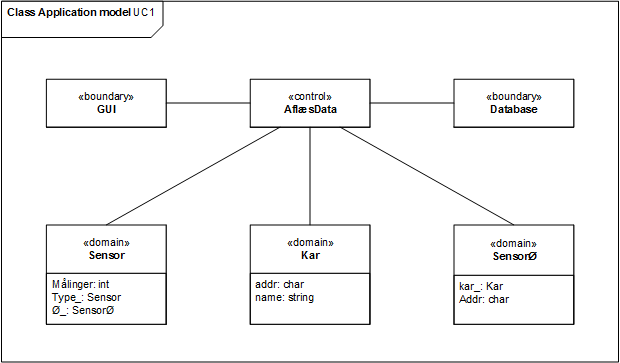
\includegraphics[width=0.8\textwidth]{Systemarkitektur/KlasseDiagrammer/1_AflaesData.PNG}
    \caption{Applikationsmodel for UC1}
    \label{fig:app_uc1}
\end{figure}

Dette klassediagram er benyttet til at identificere nødvendige klasser for at udføre use case 1.
Nedenfor er beskrives kort klassernes ansvar for use case 1.
\\\\
\textbf{AflæsData:}\\
varetager og koordinerer interaktionen mellem de interne klasser i henhold til use casen.
\\\\
\textbf{GUI:}\\
Grænseflade mellem, system go bruger, hvor brugeren aflæser de målte data. 
\\\\

\subsection{Klassediagram for use case 2 - Manuel vanding}
\begin{figure}[H]
    \centering
    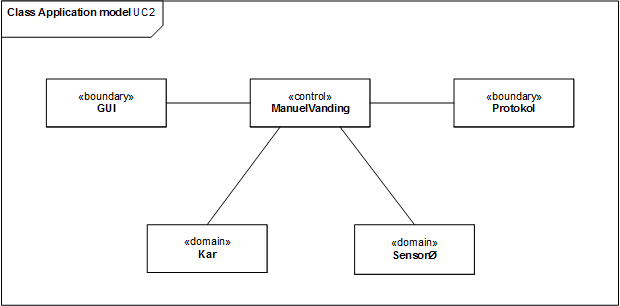
\includegraphics[width=0.8\textwidth]{Systemarkitektur/KlasseDiagrammer/2_ManuelVanding.PNG}
    \caption{Applikationsmodel for UC2}
    \label{fig:app_uc2}
\end{figure}

Dette klassediagram er benyttet til at identificere nødvendige klasser for at udføre use case 2.
Nedenfor er beskrives kort klassernes ansvar for use case 2.
\\\\
\textbf{Manuel vanding:}\\
varetager og koordinerer interaktionen mellem de interne klasser i henhold til use casen.
\\\\
\textbf{GUI:}\\
Grænseflade mellem, system go bruger, hvor brugeren kan aktivere den manuelle vanding. 
\\\\
\textbf{Protokol:}\\
Bussystem, der kommunikerer med vores hardware, så manuel vanding kan aktiveres.
\\\\

\subsection{Klassediagram for use case 3 og 4 - Indtast data}

\begin{figure}[H]
    \centering
    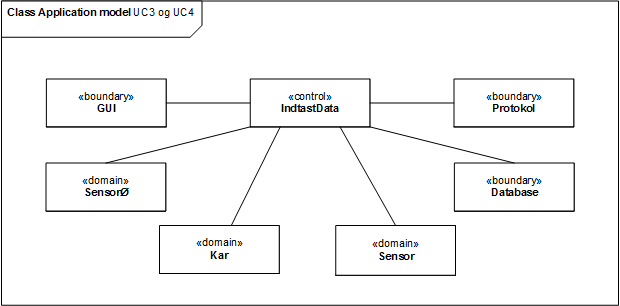
\includegraphics[width=0.8\textwidth]{Systemarkitektur/KlasseDiagrammer/3+4_IndtastData.PNG}
    \caption{Applikationsmodel for UC3 og UC4}
    \label{fig:app_uc2}
\end{figure}

Dette klassediagram er benyttet til at identificere nødvendige klasser for at udføre use case 3 og 4.
Nedenfor er beskrives kort klassernes ansvar for use case 3 og 4.
\\\\
\textbf{IndtastData:}\\
varetager og koordinerer interaktionen mellem de interne klasser i henhold til use casen.

\textbf{GUI:}\\
Grænseflade mellem, system go bruger, hvor brugeren Indtaste de ønskede data. 
\\\\

\textbf{Database:}\\
Grænseflade mellem GUI og FlexPMS, hvor de  indtastede data bliver gemt. 
\\\\

\subsection{Klassediagram for use case 5 og 6 - Kar manipulation}

\begin{figure}[H]
    \centering
    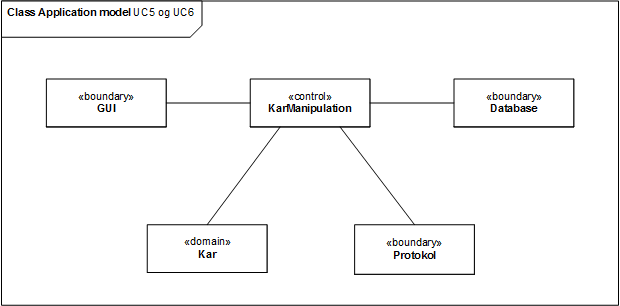
\includegraphics[width=0.8\textwidth]{Systemarkitektur/KlasseDiagrammer/5+6_KarManipulate.PNG}
    \caption{Applikationsmodel for UC5 og UC6}
    \label{fig:app_uc2}
\end{figure}

Dette klassediagram er benyttet til at identificere nødvendige klasser for at udføre use case 5 og 6.
Nedenfor er beskrives kort klassernes ansvar for use case 5 og 6.
\\\\
\textbf{KarManipulation:}\\
Varetager og koordinerer interaktionen mellem de interne klasser i henhold til use casen.
\\\\
\textbf{GUI:}\\
Grænseflade mellem, system go bruger, hvor brugeren kan oprette og slette kar. 
\\\\

\textbf{Database:}\\
Grænseflade mellem GUI og FlexPMS, hvor det forskellige kar bliver gemt med deres data. 
\\\\